\subsection{Estimation of roll damping from roll decay tests}
\label{se:experimental_estimation}
The roll decay test has the benefit of that both roll damping and the natural frequency $\omega_0$ can be observed, but the drawback that roll damping at only this one frequency can be obtained. In order to extract roll damping parameters from the roll decay tests, parameters in the cubic, quadratic or linear roll decay models should be identified. The roll angle is measured during the roll decay tests. The system identification is defined as finding the parameters that produce a simulated roll signal that best fits the roll decay test measurement. 
%To evaluate the performed tests, a modified version of the PIT approach is developed. 
%The ``Derivation approach" has the advantage of being very much faster than the ''Integration approach" but also the disadvantage of needing to calculate the numerical derivatives which for measurement data also requires some low pass filtration. The "Integration approach" may however also have a disadvantage of not converging.



%Peter Piehl \parencite{henry_peter_piehl_ship_nodate} shows an analytical solution %to the linear model in equation \ref{eq:roll_decay_equation_himeno_linear}, %where the natural frequency of the motion is obtained by:
%\begin{equation}
\omega_{0} = \sqrt{\frac{C}{A_{44}}}
\end{equation}

%
%The roll damping and the natural frequency can be made non dimensional using %the following expressions \parencite{himeno_prediction_1981}: 
%\begin{equation} \label{eq:B44_hat_equation}
B_{44 hat} = \frac{\sqrt{2} \sqrt{\frac{beam}{g}} \operatorname{B_{44}}\left(\dot{\phi}\right)}{2 Disp beam^{2} \rho}
\end{equation}

%\begin{equation} \label{eq:omega_hat_equation}
\omega_{hat} = \frac{\sqrt{2} \omega \sqrt{\frac{beam}{g}}}{2}
\end{equation}

%The ordinary differential equations for roll motion in equation \ref{eq:roll_decay_equation_cubic}, \ref{eq:roll_decay_equation_himeno_quadratic} and \ref{eq:roll_decay_equation_himeno_linear} are solved numerically using Explicit Runge-Kutta method of order 5(4). 

%Figure \ref{fig:analytical} shows a comparison for the linear model between this kind of numerical solution and the exact analytical solution \parencite{henry_peter_piehl_ship_nodate}. It seems that the numerical solution agrees well with the analytical. 

%\begin{figure}[h]
%    \centering
%    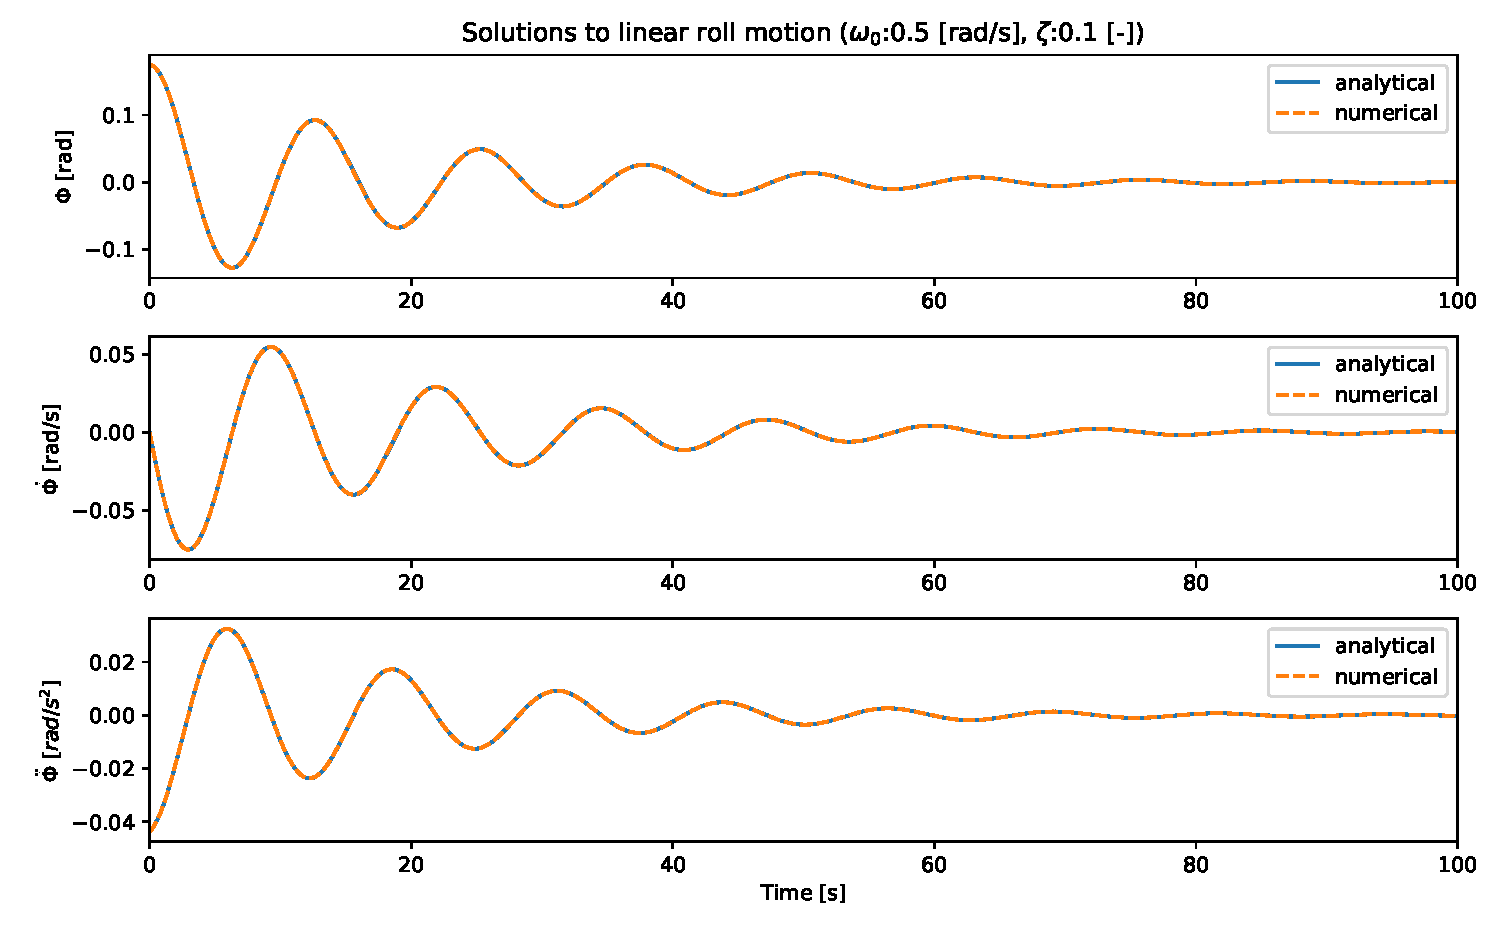
\includegraphics[width=\columnwidth]{figures/analytical.pdf}
%    \caption{Analytical and numerical solution to the linear model}
%    \label{fig:analytical}
%\end{figure}


%\subsection{Parameter Identification Technique}
%\label{se:PIT}
Two different solution approaches have been investigated for the system identification, i.e., the "Derivation approach" (referred to as PIT in \parencite{imo_1200_2006}) and the "Integration approach" which is similar to what \parencite{soder_assessment_2019} used. In the ``Derivation approach" the first and second roll time derivatives are calculated numerically so that the parameters in the models are the only unknowns and the optimal parameters that gives the best fit can simply be determined using a least square fit.
In the ``Integration approach" the parameters are found by solving a nonlinear least-squares problem using the least-square method. This approach requires that ordinary differential equation is solved for many ``guessed" sets of parameters till the solution converges.

It should be noted that even though the approach could well handle roll equations with higher order of non-linearities in the damping term as well as a non-linear restoring term, the limited amplitudes at which the roll decay tests were conducted cannot motivate advantages of higher order models. A validation of the developed parameter identification method has been conducted by checking that parameters from simulated signals with the linear, quadratic and cubic model  (where the parameters are already known) can be identified correctly. 
The goodness of the fit is described using the coefficient of determination:
\begin{equation} \label{eq:R2}
%R^2=1-\frac{SS_{res}}{SS_{tot}}
R^2=1-\frac{\sum\limit_{i=1}^{n}(y_i-\hat{y}_i)^2}{\sum\limit_{i=1}^{n}(y_i-\bar{y})^2}
\end{equation}
where $y_i$, $\bar y$, $\hat{y}_i$ represents the motion angle $\phi$, mean of $\phi$ from the model tests, and estimated $\phi$ by the system identification method, while they represent the damping coefficients in the Section 3.      


